\chapter{Essentials}


\section{Cosmic Radiation}
The cosmos is filled with particles of many kinds and sources.
Whereas the direction of travel of charged particles is constantly bent by electromagnetic fields on their journey through space,
uncharged particles such as gamma rays preserve their direction during their voyage.
These circumstances allow the sources to be identified.
Source specific characteristics can be measured by determining the particle's properties.

\begin{figure}
    \centering
    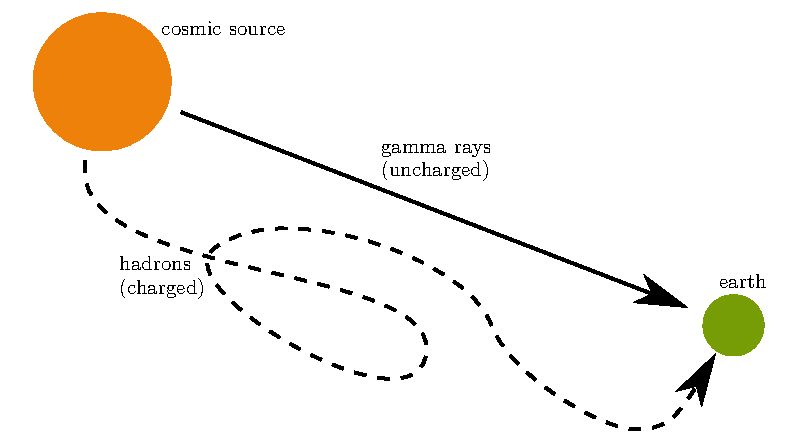
\includegraphics[scale=1]{Plots/Cosmic_Radiation.pdf}
    \caption{Uncharged particles propagate in straight lines and charged particles propagate unpredictably through space.}
    \label{fig:cosmic_radiation}
\end{figure}

Neither gamma particles nor hadrons can pass through the Earth's atmosphere and for this reason collide with it.
In this way the cosmic particle transfers some of its energy to its collision partner.
This causes an air shower by reason of the high energies in the \si{\mega\eV} range involved.
Since the speed of light in air is lower than in space,
some particles in an air shower can be faster than the speed of light in air
without violating the speed of light in vacuum;
these particles emit a cone of Cherenkov radiation.
When a high energy cosmic particle interacts with the atmosphere,
a short flash of Cherenkov light can be detected at ground-level \cite{basic_physics}.

\begin{figure}
    \centering
    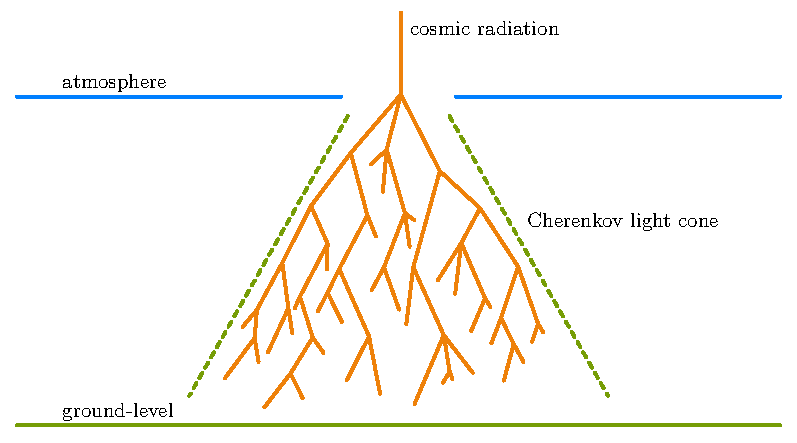
\includegraphics[scale=1]{Plots/Air_Shower.pdf}
    \caption{Cosmic particles cause air showers in the atmosphere by colliding with it. These showers emit Cherenkov light}
    \label{fig:air_shower}
\end{figure}


\section{The First G-APD Cherenkov Telescope}
Among other telescopes, the First G-APD Cherenkov Telescope (FACT) on La Palma records these light flashes.
It uses Geiger-mode avalanche photodiodes (G-APDs) as optical sensors for a test benchmark of this technology.
With a comparatively small mirror surface area of \num{9.5}\,\si{\meter²} it has operated since \num{2011}
and takes images of air showers caused by cosmic radiation in the TeV energy range \cite{FACT}.

The \num{1440} camera pixels form a hexagonal grid.
This hexagonal pixel structure represents a challenge for further image processing
as software for image classification was developed for images with square pixels.
Therefore, the camera image has to be transformed by using the pixel IDs
to map from the hexagonal to a quadratic grid structure \cite{hexagonal}.
Skewing the image by translating it to a different coordinate system and padding it with empty pixels
enables further processing without developing special software.
One drawback of this procedure is the loss of some direct neighborhood information for every pixel
(hexagonal: \num{6} neighbors, square: \num{2}\,times \num{4} equivalent neighbors).

\begin{figure}
    \centering
    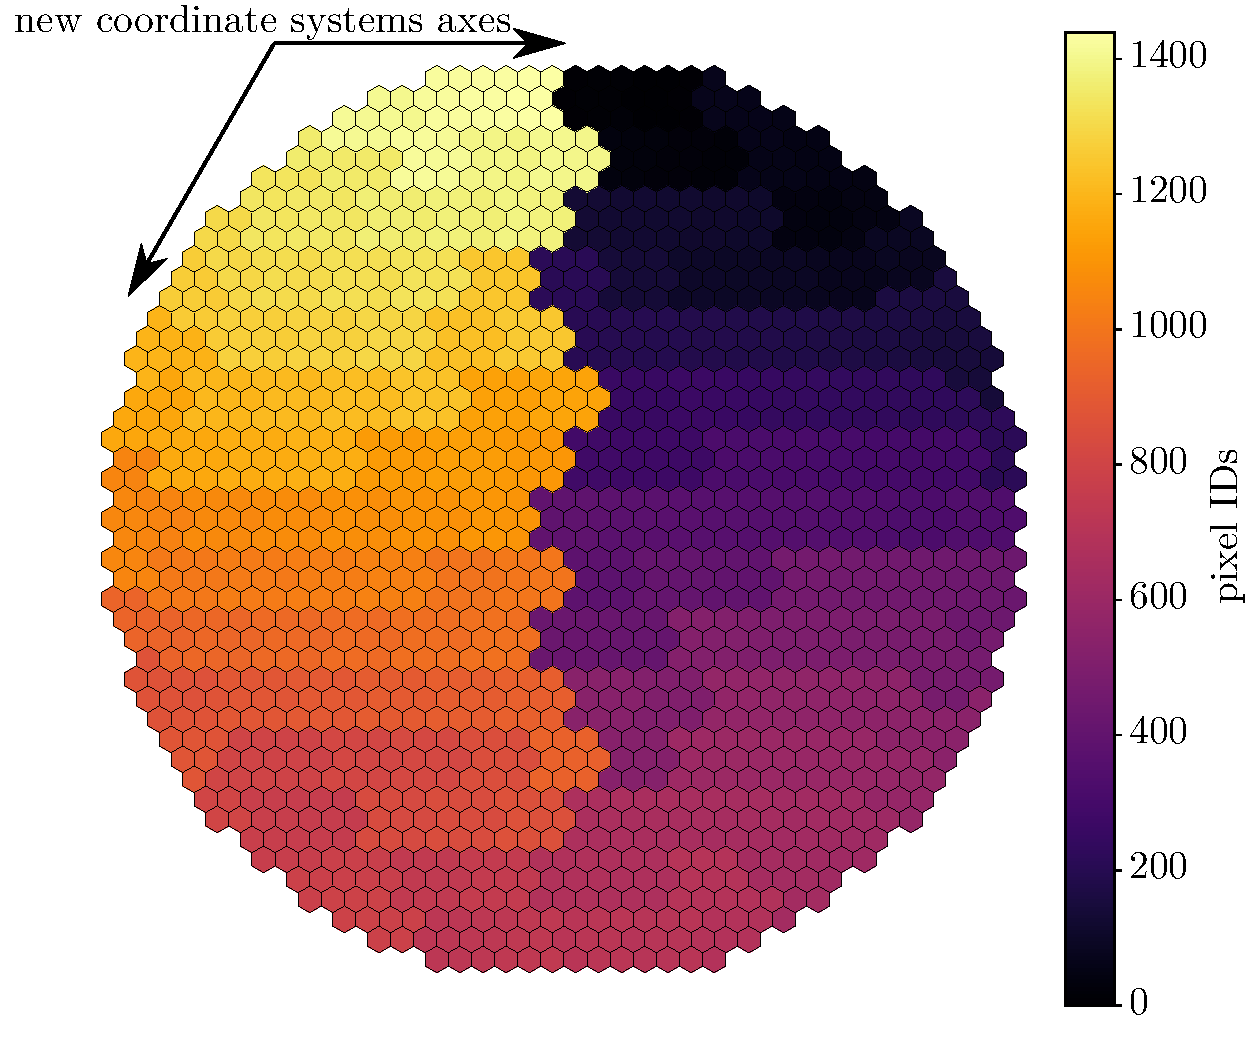
\includegraphics[width=100mm]{Plots/FACT_Image.pdf}
    \caption{Translating the FACT camera image to a new coordinate system by using the axes shown allows a transformation from a hexagonal to a square grid structure.}
    \label{fig:fact_image}
\end{figure}

\begin{figure}
    \centering
    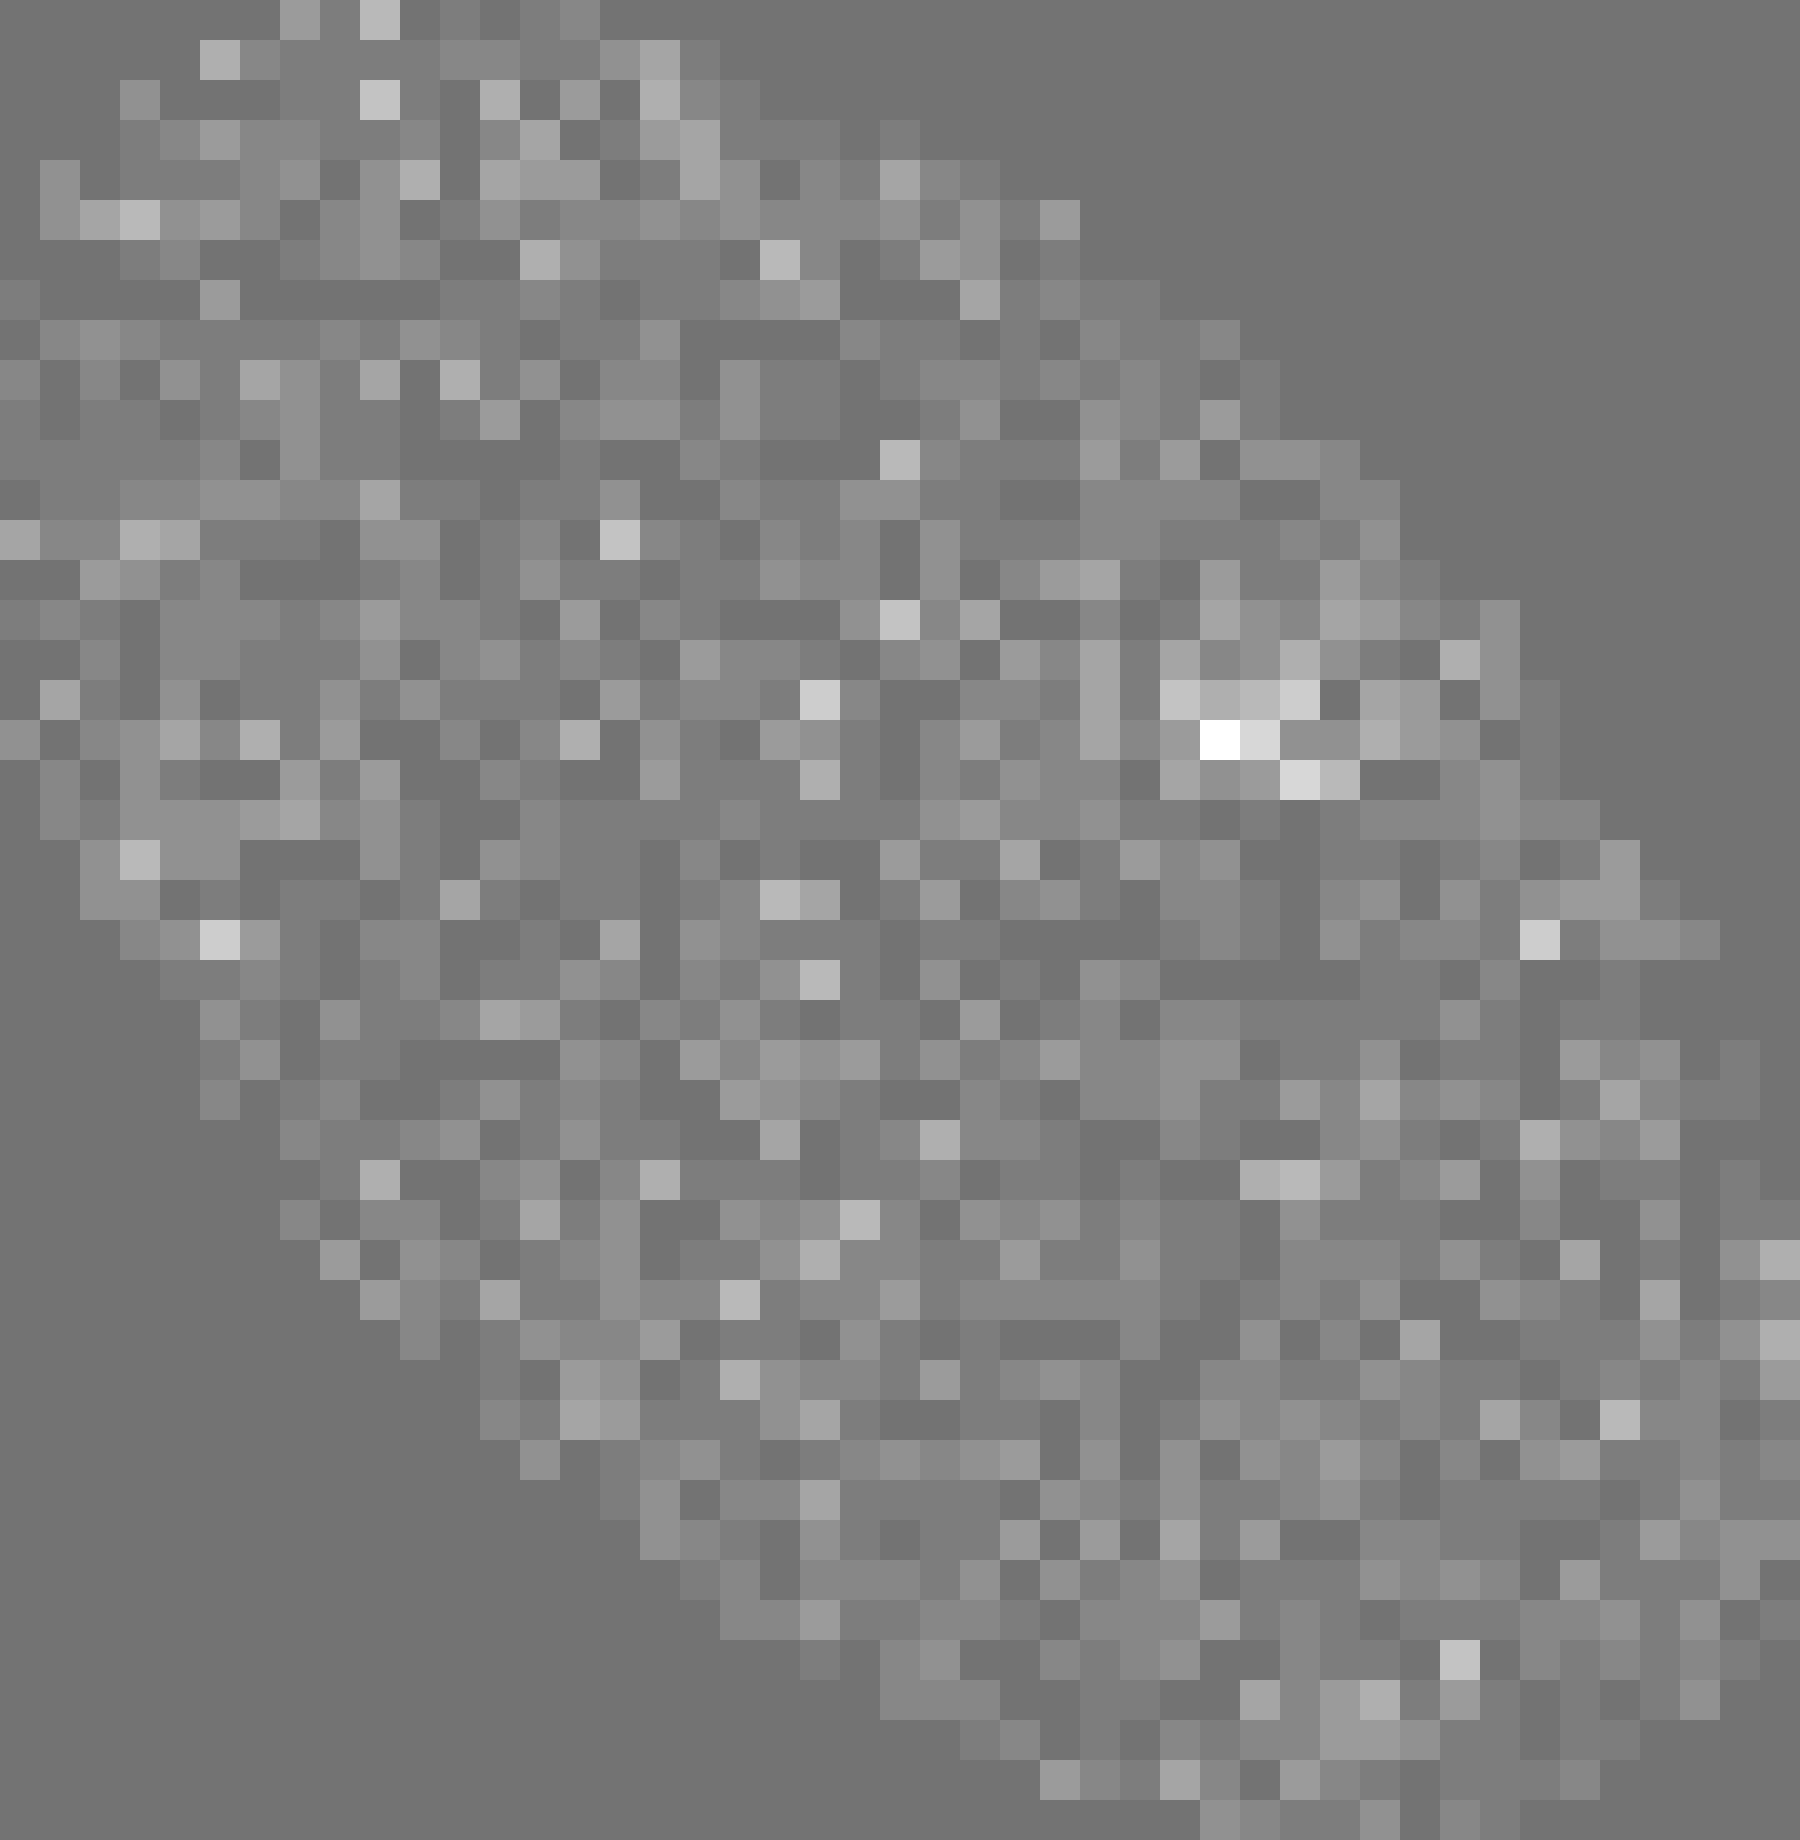
\includegraphics[width=60mm]{Plots/Preprocessed_Image.png}
    \caption{The transformed camera image will be padded with zeros and has a final size of \num{45} by \num{46} pixels.}
    \label{fig:preprocessed_image}
\end{figure}



\section{Convolutional Neural Networks}
In recent years Deep Learning has evolved at an incredible rate and made impressive progress in image classification tasks.
In light of this, this thesis tests the utility of Convolutional Neural Networks (CNN) for classifying the skewed camera images
by the particle type which induced the air shower.
For differentiating between images caused by gammas or hadrons, there are many possible architectures for the CNN.
With this in mind, every architecture is composed of layers each with a different role.
The image will then be passed from layer to layer, undergoing transformations at each one.

\begin{itemize}
\item Convolution layers (denoted in the plots by \enquote{c}) act as feature generators.
These layers allow for the translation invariant recognition of patterns.

\item Pooling layers reduce the feature space by selecting the most important features.
They follow convolution layers and will not be denoted in the plots.

\item Fully-connected layers (denoted by \enquote{f}) will make up the final layers of the net.
They combine the computed features and classify the image.
\end{itemize}

\begin{figure}
    \centering
    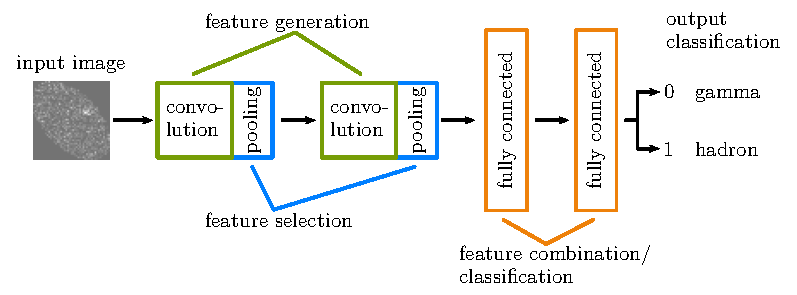
\includegraphics[scale=1]{Plots/CNN_Example.pdf}
    \caption{The input image will be transformed by each layer and passed onto the next one until it finally reaches the output layer, which classifies the image.}
    \label{fig:cnn_example}
\end{figure}

To minimize overfitting behavior and maximize generalizability of the network, different approaches can be used.
To attain evenly-distributed pixel values,
each batch of images fed into the network is preprocessed to have a mean of \num{0} and a standard deviation of \num{1} (batch normalization).

At the expense of longer training times, dropout layers (\enquote{d}) can be inserted after any layer.
This will drop some of the information flowing through the network
and force it to learn distributed representations of every feature, making the network more robust.

To enable deeper networks and faster training, pretraining will be employed.
After training shallow networks for a short time, a new, untrained layer will be attached.
This process will be repeated until the network's growth reached its final depth.
While most of the layers only have to adapt slightly,
the new layers can adjust their behavior according to the pretrained network quickly.
Additional insights into Convolutional Neural Networks and Deep Learning can be found in Ian Goodfellow's book \enquote{Deep Learning} \cite{deeplearning}.

For implementing the layers and the architectures Google's Python library \texttt{TensorFlow} \cite{tensorflow} has been used.
GPUs were used for training
to take advantage of their parallel computing capabilities and thereby cutting down the training time.
This results in training times fluctuating between \num{15}\,\si{\minute} and \num{90}\,\si{\minute} for a single network.
